\documentclass[12pt, a4paper]{report} % Defines the font size and the paper format

\usepackage[utf8]{inputenc}
\usepackage[T1]{fontenc}
\usepackage{textcomp}


\usepackage{amsmath, amssymb, amsfonts} % Standard AMS packages
\usepackage{amsthm}           % For theorem environments
\usepackage{geometry}         % Customize page geometry
\usepackage{setspace}         % To set line spacing
\usepackage{graphicx}
\usepackage[ngerman, english]{babel}


\usepackage[hidelinks]{hyperref}
\usepackage{graphicx, xcolor}

\usepackage{pgfplots}
\usepackage{pdflscape}

\usepackage{pgfgantt}
\usepackage{float}

\usepackage{color}
\usepackage{xcolor}
\usepackage{listingsutf8}

\definecolor{codeBackground}{rgb}{.95,0.95,0.95}

\newcommand{\coloredlstinline}[2]{\colorbox{codeBackground}{\lstinline[language=#1]|#2|}}

\lstset{basicstyle=\ttfamily\footnotesize,breaklines=true}
\definecolor{tangoSkyBlue}{RGB}{32, 74, 135}
\definecolor{tangoOrange}{RGB}{206, 92, 0}
\definecolor{tangoChameleon}{RGB}{78, 154, 6}
\definecolor{tangoButter}{RGB}{196, 160, 0}

\lstdefinelanguage{Rust}{
	basicstyle=\normalsize\ttfamily,
	keywords=[0]{let, pub, struct, enum, type, impl, fn, const, mut, extern, use, mod, continue, break, loop, while, crate, true, false, bool, char, str, u8, i8, u16, i16, u32, i32, u64, i64, u128, i128, usize, isize, f32, f64, match, switch, if, else, return, trait, ref, unsafe, union, for, in, dyn, where, default, as, move, static},
	keywords=[1]{|, -, !, ?, \&, *, Err, Ok, None, Some, self},
%	keywords=[2]{println!, writeln!, print!, write!},
	otherkeywords={!, ?, |, -, \&, *, \_},
	morekeywords=[1]{!, ?, |, -},
	sensitive=true,
	morecomment=[l]{//},
	morecomment=[s]{/*}{*/},
	morestring=[b]',
	morestring=[b]",
	morestring=[s][\color{tangoOrange}]{'}{a},
	alsoletter={! ? | - \& * \_},
	moredelim = [l][\color{tangoOrange}]{\#}
}

\lstdefinelanguage{help}{
	basicstyle=\ttfamily\footnotesize,
	keywords=[0]{default},
	keywords=[1]{|, -, !, ?, \&, *, Err, Ok, None, Some, self},
	%	keywords=[2]{println!, writeln!, print!, write!},
	otherkeywords={!, ?, |, -, \&, *, \_},
	morekeywords=[1]{!, ?, |, -},
	sensitive=true,
	morecomment=[l]{//},
	morecomment=[s]{/*}{*/},
	morestring=[b]',
	morestring=[b]",
	morestring=[s][\color{tangoOrange}]{'}{a},
	alsoletter={! ? | - \& * \_},
	moredelim = [l][\color{tangoOrange}]{\#}
}

%\usepackage{sourcecodepro}
%\usepackage{fontspec}
%\setmonofont{CMU Typewriter Text}
\lstset{
	backgroundcolor=\color{codeBackground},
	basicstyle=\ttfamily,
	breakatwhitespace=false,
	breaklines=true,
	captionpos=b,
	extendedchars=true,
	language=Rust,
	keywordstyle=\bf,
	showspaces=false,
    showstringspaces=false,
	showtabs=false,
	tabsize=4,
	aboveskip=5mm,
	belowskip=5mm,
	numbers=left,
	numberstyle=\tiny\color{gray},
	keywordstyle=[0]\bfseries\color{tangoSkyBlue},
	keywordstyle=[1]\bfseries\color{tangoOrange},
	keywordstyle=[2]\bfseries\color{tangoButter},
	commentstyle=\color{gray},
	stringstyle=\color{tangoChameleon},
	extendedchars=true,
	literate={ä}{{\"{a}}}1 {ö}{{\"{o}}}1 {ü}{{\"{u}}}1 {ß}{{\ss}}1,
	columns=fixed,
	keepspaces=true,
	breaklines=true,
	breakatwhitespace=true
}
\lstset{
	backgroundcolor=\color{codeBackground},
	breakatwhitespace=false,
	breaklines=true,
	captionpos=b,
	extendedchars=true,
	language=help,
	keywordstyle=\bf,
	showspaces=false,
	showstringspaces=false,
	showtabs=false,
	tabsize=4,
	aboveskip=5mm,
	belowskip=5mm,
	numbers=left,
	numberstyle=\tiny\color{gray},
	keywordstyle=[0]\bfseries\color{tangoSkyBlue},
	keywordstyle=[1]\bfseries\color{tangoOrange},
	keywordstyle=[2]\bfseries\color{tangoButter},
	commentstyle=\color{gray},
	stringstyle=\color{tangoChameleon},
	extendedchars=true,
	literate={ä}{{\"{a}}}1 {ö}{{\"{o}}}1 {ü}{{\"{u}}}1 {ß}{{\ss}}1,
	columns=fixed,
	keepspaces=true,
	breaklines=true,
	breakatwhitespace=true
}


\newcommand{\coloredlstinlinev}[2]{\colorbox{codeBackground}{\lstinline[language=#1]|#2|}}
\newcommand{\rustcinline}[1]{\coloredlstinline{rust}{#1}}
\newcommand{\rustcinclude}[3]{\lstinputlisting[language=rust,caption={#2},label={#1}]{#3}}
\newcommand{\rustcincludeml}[3]{\lstinputlisting[xleftmargin=1.2em,language=rust,caption=#2,label=#1]{#3}}

\newcommand{\helpinclude}[3]{\lstinputlisting[language=help,caption={#2},label={#1}]{#3}}

\newcommand{\javacinline}[1]{\coloredlstinline{java}{#1}}
\newcommand{\javacinclude}[3]{\lstinputlisting[language=java,caption={#2},label={#1}]{#3}}

\newcommand{\cscinline}[1]{\coloredlstinline{{[Sharp]C}}{#1}}

\newcommand{\ccinline}[1]{\coloredlstinline{c}{#1}}
\newcommand{\ccinclude}[3]{\lstinputlisting[language=c,caption={#2},label={#1}]{#3}}
\newcommand{\ccincludeml}[3]{\lstinputlisting[xleftmargin=1.2em,language=c,caption=#2,label=#1]{#3}}

\newcommand{\monospaceinclude}[3]{\lstinputlisting[basicstyle=\footnotesize,language=bash,caption=#2,label=#1]{#3}}
\newcommand{\monospaceinline}[1]{\coloredlstinline{bash}{#1}}
%\renewenvironment{rustc}{\begin{lstlisting}[language=rust]}{\end{lstlisting}}

\usepackage{tikz-uml}

\usetikzlibrary{pgfplots.statistics}        % to draw `boxplot's

% strange bug with arrows.meta
% You can't use `\unskip' in vertical mode.
% https://tex.stackexchange.com/questions/298904/strange-tikz-problem-memoir-vs-xcolor-vs-tikz/299001
\newbox\tempbox
\newif\ifdebug
\debugtrue
\makeatletter
\def\pgfmathsetlength #1#2{\expandafter \pgfmath@onquick #2\pgfmath@
        {\ifdebug\typeout{HERE\detokenize{#1}\detokenize{#2}}\fi
                \setbox\tempbox\hbox{\pgfmath@selectfont#1#2\relax\expandafter}\expandafter#1\the #1\relax
                \ifdebug\typeout{#1=\the#1}\fi}%
        {\pgfmathparse {#2}\ifpgfmathmathunitsdeclared #1\pgfmathresult mu\relax
                \else #1\pgfmathresult pt\relax \fi }\ignorespaces }
\makeatother


\usetikzlibrary{backgrounds,scopes,arrows, arrows.meta, positioning, shadows}

\makeatletter




% #1 label
% #2 Requirement Number
% #3 Name
% #4 Description
\newcommand{\requirement}[4]{%
	\expandafter\edef\csname{}req_number_#1\endcsname{#2}
	\expandafter\edef\csname{}req_name_#1\endcsname{#3}
	\expandafter\edef\csname{}req_desc_#1\endcsname{#4}%
}



\newcommand{\reqNumber}[1]{\csname{}req_number_#1\endcsname}
\newcommand{\reqName}[1]{\csname{}req_name_#1\endcsname}
\newcommand{\reqDesc}[1]{\csname{}req_desc_#1\endcsname}

\newcommand{\captionsource}[1]{\caption*{\footnotesize{Quelle: #1}}}

\newcommand{\reqLabel}[1]{\label{req:#1}}
\newcommand{\reqRef}[1]{[R\hyperref[req:#1]{\reqNumber{#1}}]}
\newcommand{\reqHeader}[1]{Requirement \reqNumber{#1}: \reqName{#1}}
\newcommand{\reqNameRef}[1]{\reqName{#1} \reqRef{#1}}


\newcommand{\reqItem}[1]{\item \textbf{\reqHeader{#1}}\\\reqDesc{#1}}
\newcommand{\reqItemL}[1]{\item \reqLabel{#1} \textbf{\reqHeader{#1}}\\\reqDesc{#1}}


\makeatother

\newcommand{\todo}[1]{\textcolor{red}{TODO: #1}}


%--------------------------------------------------------------------
%--- Title, author, date
%--------------------------------------------------------------------

\newcommand{\theuniversity}{
  \begin{figure}[h]
    \centering
    
\includegraphics[width=.5\textwidth]{brunel.jpg}
  \end{figure}}
\newcommand{\thecollege}{College of Engineering, Design and Physical Sciences, Electronic and Computer Engineering}
\newcommand{\thedepartment}{Distributed Computing Systems Engineering}
%\newcommand{\thecoursetitle}{Master Thesis - Interim Report}
\newcommand{\thecoursetitle}{Interim Report}
\newcommand{\thestudent}{Michael Watzko}
\newcommand{\thestudentid}{1841795}
\newcommand{\thesupervisor}{Dr. Paul Kyberd}
\newcommand{\theyear}{2019}
\newcommand{\thetitle}{ Conception and realization of a distributed and automated computer vision pipeline}

%--------------------------------------------------------------------
%--- Global page geometry and layout
%--------------------------------------------------------------------

% Define the page margins
\geometry{
  left=40mm,
  right=25mm,
  bindingoffset=0mm, 
  top=25mm,
  bottom=25mm
}

%---------------------------------------------------------------------
%--- Theorem environments
%---------------------------------------------------------------------

% Theorem counter is subordinate to chapter; all theorem-like
% environments are using the same counter
\theoremstyle{plain}
\newtheorem{theorem}{Theorem}[chapter]          
\newtheorem{lemma}[theorem]{Lemma}
\newtheorem{proposition}[theorem]{Proposition}
\newtheorem{corollary}[theorem]{Corollary}

\theoremstyle{definition}
\newtheorem{definition}[theorem]{Definition}
\newtheorem{remark}[theorem]{Remark}

%---------------------------------------------------------------------
%--- Bibliography
%---------------------------------------------------------------------

\usepackage[style=numeric, minnames=3,
            doi=false, url=false, isbn=false,
            sorting=none, backend=biber]{biblatex}

\addbibresource{bibliography.bib}

%---------------------------------------------------------------------
%--- Document begins here
%---------------------------------------------------------------------

\begin{document}
\onehalfspacing

%---------------------------------------------------------------------
%--- Title page
%---------------------------------------------------------------------

\begin{titlepage}
\center

% Name of university, college, department and degree
\textsc{\LARGE \theuniversity} \\[0.5cm] 
\textsc{\large 
\thecollege \\ [1.0cm]
\thedepartment} \\[1.5cm]
\textsc{\Large \textbf{\thecoursetitle}} \\[1.8cm]

% Project title
\rule{\linewidth}{0.25mm} \\[0.5cm]
{ \Large\textbf{\thetitle} } \\
\rule{\linewidth}{0.25mm} \\[3.5cm]

% Student name, student number and supervisor
\begin{minipage}{0.4\textwidth}
\begin{flushleft} \large
\textbf{\thestudent} \\
\thestudentid
\end{flushleft}
\end{minipage}
~
	\begin{minipage}{0.4\textwidth}
\begin{flushright} \large
\emph{Supervisor:} \\
\thesupervisor
\end{flushright}
\end{minipage}\\[4cm]

% Year
{\large Date of Submission: {\selectlanguage{english}\today}} \\[3cm] 

\vfill % Fill the rest of the page with whitespace
\end{titlepage}
\newpage

%---------------------------------------------------------------------
%--- Front matter
%---------------------------------------------------------------------

\setstretch{1.5}
\pagenumbering{roman}

% to utf8: ö

\chapter*{Abstract} % The asterisk prevents this file from being labelled as a chapter.
%\addcontentsline{toc}{chapter}{Abstract}
 
 

A short summary of what the project is about.

\todo{.}

schedule large work items

special hardware needs

automation and highly customizable pipeline

focus on easy setup  and low maintenance

~\\
Keywords: Software, Architecture, Events, Messaging, Filesystem, Distributed, Coordination, Docker, Spring Boot, REST, Angular, Typescript
\chapter*{Declaration of Independence \todo{hehe}}

\chapter*{Abstract}

\tableofcontents
\newpage
%---------------------------------------------------------------------
%--- Main part of thesis
%---------------------------------------------------------------------

\pagenumbering{arabic}

%\input{chapter_A}
\chapter{Introduction}

Since the industrial revolution, humans strive for more automation in the industry as well as in the every day life.
What was at first a cost saving measurement in factories, now also is a differentiation method for products.
A new product must prove a higher level comfort to the customer than the previous generation as well as all the competitors.
As such, the ambitions of the industry are focused on increasing the value of their products for the customer.

The automotive industry is one of the prime examples of this.
Never was traveling from one place to another as comfortable as nowadays.
Aspects like an elegant interior design, comfortable seats, air conditioning, entertainment systems and safety measurements need to be considered by car manufacturers to be competitive these days. 
The next luxury enhancement will be the autonomously driving vehicle.
No longer shall the owner of a car steer it, but instead the car becomes his or hers personal chauffeur, driving the optimal route, the most comfortable way and being more reliable and safer than any human ever could.

The reason, autonomously driving cars are not common already, is their big complexity increase.
Compared to already established technologies like parking assistants, entertainment systems or more efficient engine controllers, letting a computer reliably understand a certain traffic situation requires masses of input data and complex algorithms to process.
As such, the problem itself becomes massive and cannot be solved that easily.
So the industry has no choice than to divide this into many small pieces and work out solutions step by step.

The MEC-View research project explorers one such step: whether and how to include external, steady mounted sensors in the decision finding process for partially autonomous vehicles in situations where onboard sensors are insufficient.
%As additional restriction, decisions made by autonomous vehicles  are not allowed to disrupt the surrounding traffic flow otherwise phenomens like the \todo{Phantomstau} could be caused by them.
To not disrupt traffic flow with non-human behavior, one needs to study and thereby watch human traffic.
Automatically analyzing traffic from video footage requires a lot of computation power and can be further optimized by specialized hardware such as GPUs\footnote{Graphics Processing Units}.

This thesis will conceptualize and realize a distributed and automated computer vision pipeline which is in this case used to analyzes traffic flow within video footage.
Compared to an existing but highly manual workflow, the new system shall help to utilize the available hardware more efficiently by reducing idle times.
Stage transitions and basic scheduling shall be automated to allow a user to plan and execute multiple projects ahead of time and in parallel.
%The current, highly manual workflow, can lead to a lot of idle time inbetween user intervention.

%The available hardware resources shall be utilized more efficiently, as well as time that is required by humans to monitor the system.


\newpage
\section{MEC-View}

%\todo{shorten!?}

The MEC-View research project\cite{mecview:main} - funded by the German Federal Ministry for Economic Affairs and Energy - aims to supplement the field of view of automated driving cars with road-side sensor data using 5G mobile communication. The sensor information is merged into an environment model on the so-called Mobile Edge Computing (MEC) server. This server is directly attached to the radio station to ensure low latency environment model updates.

The project is tested at an intersection in Ulm, Germany.
Currently, there are 15 lidar and video sensors installed.
Those sensors send their detections to the (MEC) server.
A fusion-algorithm merges those detections into one environment model and sends it back to the (MEC) server and to the automated cars.

Additionally, general traffic flow is analyzed to learn about movement patterns.
To do so, 4k video data is captured by an air drone from real world cross roads - not limited to the intersection in Ulm.
On each frame of such a recording, cars are detected with a neuronal network.
Detected cars are tracked throughout the video to compute the movement speed and position in time of each car.
In an analysis of all vehicles, hot-spots of high and low traffic flow can be determined.

\section{Focus}

This thesis conceptualizes and implements the distribution and automatization of a computer vision pipeline to increase the productivity in video analysis.
It is not of concern for this thesis on how to retrieve the footage or what is further archived with the results of the processed video footage.
The focus is on utilizing available hardware resources, to manage multiple projects simultaneously and to reduce the idle time of relevant hardware by slow human reaction and availability times - like working hour constraints.
An easy setup and low maintenance is also desirable.
% \todo{reaction time: like its done but not noticed for another x mins/hours, availability: work hours}


\chapter{Aims and Objectives}

This chapter will discuss the program which shall be implemented.
To do so, the problem to solve must be understood.
To gather requirements and understand the technical hurdles to overcome, this chapter is split into two sections.
First, a rough glance over the current workflow is given, which is followed by a more detailed description for the desired workflow.


\section{Current Workflow}

Currently, to analyze a video for the trajectories of  recorded vehicles, the following steps are executed manually:
\begin{enumerate}
	\item Upload the input video to a new directory on the GPU server
	\item \label{cw:ex} Execute a shell script with the video as input file and let it run (hours to days) until completed. The shell script invokes a Java Program - called TrackerApplication - with parameters on what to do with the input file and additional parameters.
	\item The intermediate result with raw detection results is downloaded to the local machine and opened for inspection. If the detection error is too high, the camera tracking has a drift or other disruptions are visible, the previous step is redone with adjusted parameters.
	\item \label{cw:st} Upload the video and intermediate result to a generic computing server and run data cleanup and analysis. This is achieved with the same Java Program as in step \ref{cw:ex}, but with different stage environment parameters.
	\item \label{cw:st_dl} Download the results, recheck for consistency or obvious abnormalities. Depending on the result, redo step \ref{cw:ex} or \ref{cw:st} with adjusted parameters again.
	\item Depending on the assignment, steps \ref{cw:st} and \ref{cw:st_dl} are repeated to incrementally accumulate all output data (such as statistics, diagrams and so on).
\end{enumerate}

Because all those steps are done manually, the user needs to check for errors by oneself.
Also, if a execution is finished or has failed early, there could be hours wasted until noticed, if the check intervals are too far apart, such as during nights or weekends.
The current approach does not scale at all for the increasing amount of projects that need to be processed.
Manually keeping track of all project states and intermediate results is tedious and has proven to be error prone.

\begin{figure}[H]
	\centering
	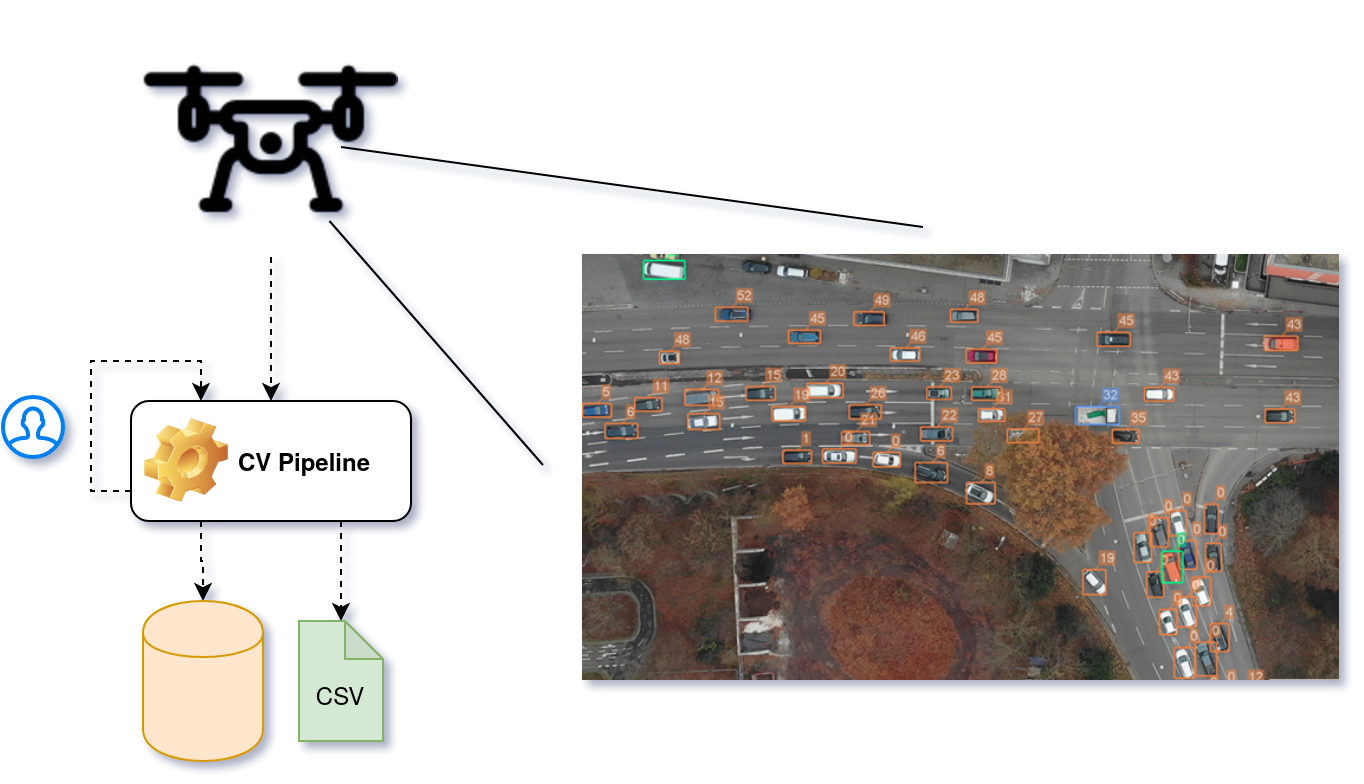
\includegraphics[width=0.9\textwidth]{overview_3.png}
	\caption{Overview of workflow}
\end{figure}

\section{Desired Workflow}
\label{workflow}
\label{workflow:desired:docker}

The desired workflow shall be supported through an user interface that provides an overview of all active projects and their current state, such as running computation, awaiting user input, failed or succeeded.

To create a new project, a predefined pipeline definition shall be selected as well as a name chosen.
Because only a handful of different pipeline definitions are expected, the creation of such does not need to happen through the user interface.
Instead, it is acceptable to have to manually edit a configuration file in such rare circumstances.

Once a project is created, the user wants to select the path to the input video.
This file has to be been uploaded to a global resource pool at this point.
The upload and download of files shall therefore also be possible through the user interface.
Because a video is usually recorded in 4k (3840 x 2160 pixels), encoded with H.264 and up to 20 minutes long, the upload must be capable of handling files which are tens of gigabytes large.

Once a pipeline is started, it shall execute the stages on the most fitting server node until finished, failed or a user input is required.
Throughout, the logs of the current and previous stage shall be accessible as well as uploading or downloading files from the current or previous stages workspace.
In addition to the pipeline pausing itself for user input, the user shall be able to request the pipeline to pause after the current stage at any moment.
When resuming the pipeline, the user might want to overwrite the starting point to, for example, redo the latest stage.

Mechanisms for fault tolerance shall detect unexpected program errors or failures of server nodes.
Server nodes shall be easily installed and added to the existing network of server nodes.
Each server node might provide additional hardware (such as GPUs), which shall be detected and provided.

For the ease of installation and binary distribution, Docker Images shall be used for running the Java Program for analyzing the videos as well the to be implemented management software.

%\todo{describe: project/pipeline -> stage?}




\section{Deliverable Requirements}

From the desired workflow, the following requirements can be extracted:

\begin{itemize}
	\item A user interface for interaction between the system and the user
	\item Storage management for global resource files as well as stage based workspaces
	\item Pipeline definition through configuration files
	\item Handling of multiple projects with independent progress and environment
	\item Reflecting the correct project state (running, failed, succeeded, paused)
	\item Log accumulation and archiving
	\item Accepting user input to update environment variables, resuming and pausing projects as well as uploading and downloading files into or from the global resource pool or a stages workspace.
	\item Assigning starting stages to the most fitting server node
	\item Detecting program errors (in a stage execution)
	\item Cope with node failures
	\item Using Docker Images as installation medium
	%Providing a Docker Image for the implemented program, preferably in an automated fashion.
%	\item \todo{.} Increase productivity without staff involvement
%	\item \todo{.} Utilize hardware in absence of staff
%	\item \todo{.} Decrease need of staff monitoring and organizing stuff
\end{itemize}

Further non-functional requirements are, that the user interface is to be implemented as Angular Web-Application using a REST API (for more details see \autoref{fundamental:angular}) for data transfer.
The system shall increase the productivity and hardware utilization, especially in times where the staff is absence.
The need to constantly monitor and interfere with the system to progress projects shall be decreased by providing automated mechanisms where possible and appropriate.

%\todo{mention? node failure resilient, easy to setup, decentralized?}

%\todo{something something agile extended as needed? \autoref{fundamental:agile}}

\begin{comment}
\subsection{Derived Requirements} \todo{.}
Requirements that are derived by looking at other requirements.


\todo{functional vs nonfunctional}

Die hier gelisteten funktionalen Anforderungen beschreiben das gewünschte Verhalten des
Systems \cite[155]{goll2012methoden}.

Nichtfunktionale Anforderungen zeigen im Gegensatz zu funktionalen Anforderungen Rah-
menbedingungen bei der Umsetzung des Systems auf \cite[155]{goll2012methoden}.
\end{comment}


\subsection{Non-Requirements}

To know the requirements and expectations of a system is essential, but knowing what is not expected by the system is at least as valuable.
It prevents wasting resources, efforts and architectural specializations that will never be required or in the worst case, make further development harder by restricting available choices for the future.
 
The system to implement shall not strive to implement real time scheduling or low latency scheduling.
The expected work items are big chunks that require hours to compute, whether the assignment of the work item takes sub-seconds or several seconds is nearly unnoticeable in the overall compute time.
\chapter{State of the art}

\section{Existing software solutions}

\subsection{Hadoop MapReduce}

focus transforming a big dataset by splitting it into many jobs, distributing it onto many workers, doing a transformation on each dataset, and merging it back together (only map -> reduce)
Distributed filesystem

\subsection{Quartz}

http://www.quartz-scheduler.org/
http://www.quartz-scheduler.org/overview/

\begin{itemize}
	\item + Java
	\item - requires integration
	\item - aimed towards running a job at a given time or in certain intervals
\end{itemize}

\subsection{Jenkins / GitLab}

Pipeline file with multiple stages
a stage can be executed on a host
focused on doing a job with different inputs again and again and again
CI -> usually no user interaction

\subsection{Camunda}

https://camunda.com/

Rich Business Process Management tool, many types of tasks, steps, transitions, triggers and endpoints.
Focused upon moving a dataset along the matching path of the process.
Out of the box graphical user interface for process definition and interaction.
Allows custom external worker through queues.
Misses capability to control which task to process on which worker through fine grained filters and how to allocate and distribute resources(?).

\section{Docker}

\chapter{Outcome and Measurements}

In this chapter the outcome is measured and evaluated.

\todo{compare to initial deliverable requirements?}

\section{What did not work as expected}

\todo{timeout for events might be reached when in between the bandwidth is used by a copy of a large file and the extend signal is because of that deferred, stages that are fine are then marked as failed}

\todo{. old sections}

\section{User Authentication and Security}

One aspect that was not yet mentioned at all is user authentication and security.
Winslow is prepared in this regards because every project has an owner field and a member list and every web access check these.
An internal user repository also associates user with groups and provides defaults, such as the user and group \enquote{anonymous} and \enquote{root}, for no and full access privileges, respectively.
But at the moment, there is no user login, instead to the system all requests seem to be issued by \enquote{root}.
In the future this is planned to be replaced by an Single Sign-On implementation that uses the user accounts of our company.
Winslow is then associating a from this service given user name to an internal user and groups.
Unknown users are not allowed to see or alter anything, known users will be able to create and view their own projects and projects they are listed in as members.
%\todo{mostly planned, implemented not tested}

Winslow also supports secure HTTP (HTTPS) whenever a SSL certificate is provided\footnote{This can be seen in \autoref{appendix:winslow_installation}}.

\begin{comment}
\section{Storage}

One of the central concerns is the storage management.
The program needs to make input files available on each execution node and collect the results once the computation is complete.
There are a few main architectural strategies to approach this.
Simplified, either at a centralized location which is accessed by all execution nodes, a copy of the input files to the execution nodes or decentralized and distributed between all execution nodes and replication.
The advantages and disadvantages can depend on the specific implementation and is therefore discussed in combination of such (see \autoref{state_of_the_art}).

Further testing is required to decide whether a more complex storage system is required, or the simplicity of a centralized solution outweighs the setup and maintenance overhead.

%\subsection{Hadoop File System}
%\cite{hdfs:main}
%\cite{hdfs:doc}
%\todo{redudancy for evenly distributed}

%\subsection{NFS}
%
%local/per node cache?

\section{Coordination}

Another important concern is the coordination of the nodes.
A central coordinator with external server nodes, such as GitLab and Jenkins have, might not be sufficient for more complex and longer lasting pipelines.
The probability that the master would need to be offline while there is a stage executed, is in the scenario of the desired workflow higher than for GitLab or Jenkins, because the stage is being execution for hours or days.
Coupling stage execution plans on node availability ahead of time, as well as recovering from a sudden master failure implies additional implementation complexity.
A decentralized coordination needs to be able to do this as well, but also allows the usage of the system while a node failed or is unreachable due to maintenance.
With further prototyping and research a reasonable solution shall be found.

\section{Binary distribution}

In a time where containers are common and have proven to be usable, the installation of the binaries directly on the operating system they are executed on shall be avoided.
There shall be no manual, nor automatic but custom file copies of the binaries or images from one server to the other.
Experience shows, that without a proper management, this can easily become a mess, in which it is no longer clear, which files or images belong to which version.
At the same time, making all binaries publicly available through the Docker Hub\cite{docker:hub} is no option either.
Whether a self hosted Docker Registry\cite{docker:registry} could be the solution to this will be determined in further testing.

\section{User Interface}

Providing a useful user interface might not be important to the functionality of the system itself but for the user experience.
A bad user experience will cause a system not to be used.
It became common practice for a rich user experience to be web based and interactive with JavaScript.
For a potentially decentralized system, it is also advantageous to be able to access a disconnected node in the same manner as the remaining system, which further encourages a web based solution.
Web based solutions such as React and Angular shall therefore be investigated for being used as user interface.

\section{Requirements}

\todo{more than first defined - as expected}

\todo{lots more UI shortcuts found necessary while starting to use winslow}

\section{Architecture}

\todo{loosely coupled backend driver}\autoref{architecture:detailed}
\end{comment}

\section{High Level System Overview}

\todo{.delete?}

\autoref{architecture:high-level} shows the high level system overview of Winslow as it has been implemented by the end of this thesis.

\begin{figure}[h]
	\centering
	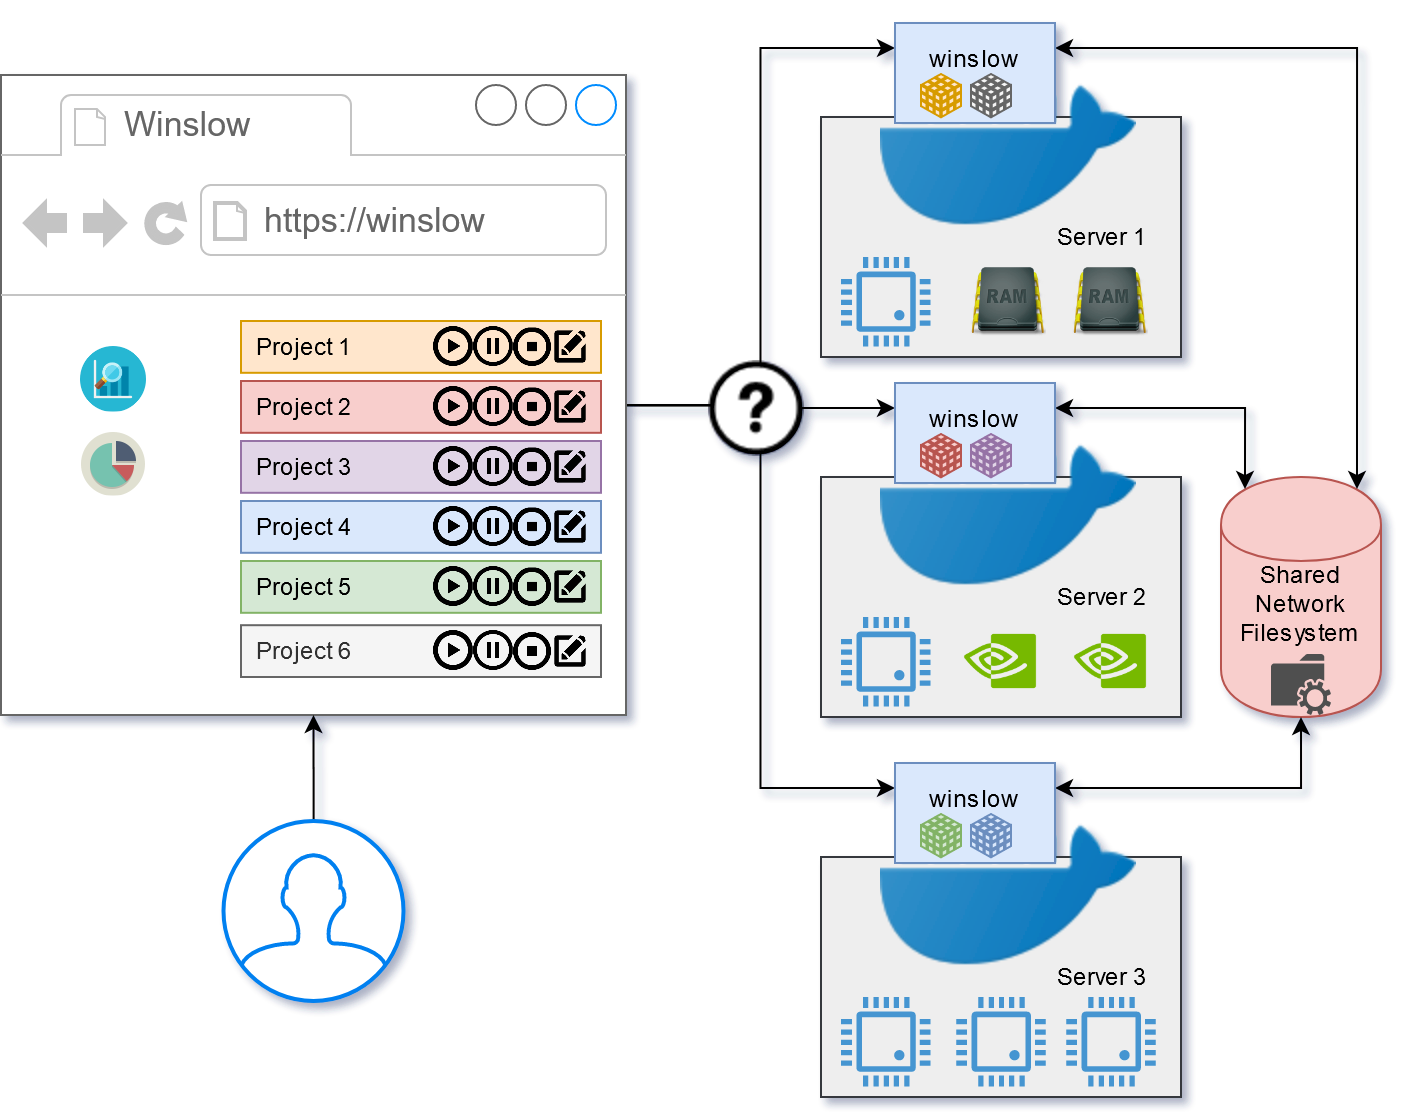
\includegraphics[width=0.8\textwidth]{architecture.png}
	\caption{High level view on the system structure}
	\label{architecture:high-level}
\end{figure}


\todo{explain what is going on in \autoref{architecture:high-level}}

\section{Failure resilience}

\todo{.delete? or polish!}

One of the initial requirements is to be resilient against node failures.
Node failures can be simulated easily by killing the Docker container of a Winslow instance.
The behaviour that is then displayed, depends on whether that killed instance was executing a stage.
If it did not, the only change is that in the Web-Application the node with its utilization reports will vanish.

But if it did execute a stage, it held locks for it.
These locks will expire, and after the additional grace period (see \autoref{message:grace_period}), the other instances will notice it, lock the affected project themselves and mark the execution as failed.
Currently, the project is then paused and user confirmation awaited.
An alternative to this could be to re-schedule the stage automatically.
\chapter{Project Management}

%\autoref{time_schedule} shows the time schedule of this work.

The project management went mostly as planned.
All deadlines regarding the implementation and deployment were met as planned.
A few of the milestones for documentation were pushed back slightly, because some parts took a bit longer to write about than anticipated at first.
But, because a time puffer at the end was considered from the beginning, the project was able finish in time.
The time schedule can be seen in \autoref{time_schedule}:

\newganttlinktype{f-m}{
	\ganttsetstartanchor{on right=1}
	\ganttsetendanchor{on left=0}
	\draw[/pgfgantt/link]
	([xshift=-.2pt]\xLeft, \yUpper) -- % xshift to fit arrow
	node[pos=.5, /pgfgantt/link label node] {\ganttlinklabel}
	(\xRight, \yLower);
}

\setganttlinklabel{f-m}{}

\begin{figure}[H]
	\centering
	\begin{ganttchart}[hgrid,vgrid,x unit = 0.4cm,y unit chart = 0.35cm,title label font=\footnotesize,group label font=\tiny,milestone label font=\tiny,bar label font=\tiny]{1}{29}
		\gantttitle{2019}{16}
		\gantttitle{2020}{13} \\
		\gantttitle{Sep}{4}
		\gantttitle{Oct}{4}
		\gantttitle{Nov}{4}
		\gantttitle{Dec}{4}
		\gantttitle{Jan}{4}
		\gantttitle{Feb}{4}
		\gantttitle{Mar}{4}
		\gantttitle{}{1} \\
		
		\ganttgroup{Interim Report}{1}{4} \\
		\ganttbar{Analyze and Understand}{1}{2} \\
		\ganttbar{Research}{1}{14} \\
		\ganttbar{Writing}{2}{4} \\
		\ganttmilestone{Submission}{4} \\ \\
		
		\ganttgroup{Master's Thesis}{5}{28} \\ \\
		\ganttgroup{Implementation}{5}{26} \\
		\ganttbar{Prototyping}{5}{16} \\
		
		\ganttbar{Decide: Architecture}{6}{8} \\
		\ganttbar{Decide: Storage Strategy}{9}{13} \\
		\ganttbar{Decide: Coordination Strategy}{14}{17} \\
		
		\ganttbar{Implement: Adapter Code}{9}{13} \\
		\ganttbar{Implement: Storage}{14}{17} \\
		\ganttbar{Implement: Coordination}{18}{22} \\
		
		
		\ganttbar{Setup CI Pipeline}{7}{8} \\
		\ganttbar{Setup Binary Distribution}{9}{12} \\
		
		\ganttbar{Implement: Corresponding UI}{10}{23} \\
		\ganttbar{Testing \& Fixing}{10}{26} \\
		
		\\
		\ganttgroup{Documentation}{9}{28} \\
		\ganttbar{Write: Architecture \& Techn.}{9}{14} \\
		\ganttbar{Write: Storage Strategy \& UI}{15}{19} \\
		\ganttbar{Write: Coordination}{20}{24} \\
		\ganttbar{Write: Conclusion}{25}{26} \\
		\ganttbar{Final corrections}{27}{28} \\
		
		\ganttmilestone{Submission}{28} \\
		
		\ganttbar{Poster Creation}{18}{23} \\
		\ganttmilestone{Poster Presentation}{23} \\
		
		\ganttlink{elem3}{elem4}
		\ganttlink{elem8}{elem9} \ganttlink{elem8}{elem11} \ganttlink{elem8}{elem19}
		\ganttlink{elem9}{elem10}  %\ganttlink{elem9}{elem12}
		\ganttlink{elem11}{elem12} %\ganttlink{elem10}{elem13}
		\ganttlink{elem12}{elem13}
		
		\ganttlink{elem14}{elem15}
		
		\ganttlink{elem19}{elem20}
		\ganttlink{elem20}{elem21}
		\ganttlink{elem21}{elem22}
		\ganttlink{elem22}{elem23}
		\ganttlink{elem23}{elem24}
	
		\ganttlink{elem25}{elem26}
	\end{ganttchart}
	\caption{Time schedule}
	\label{time_schedule}
\end{figure}


\chapter{Introducing Winslow}

\begin{wrapfigure}{r}{0.37\textwidth}
	\centering
	\vspace{-1.5cm}
	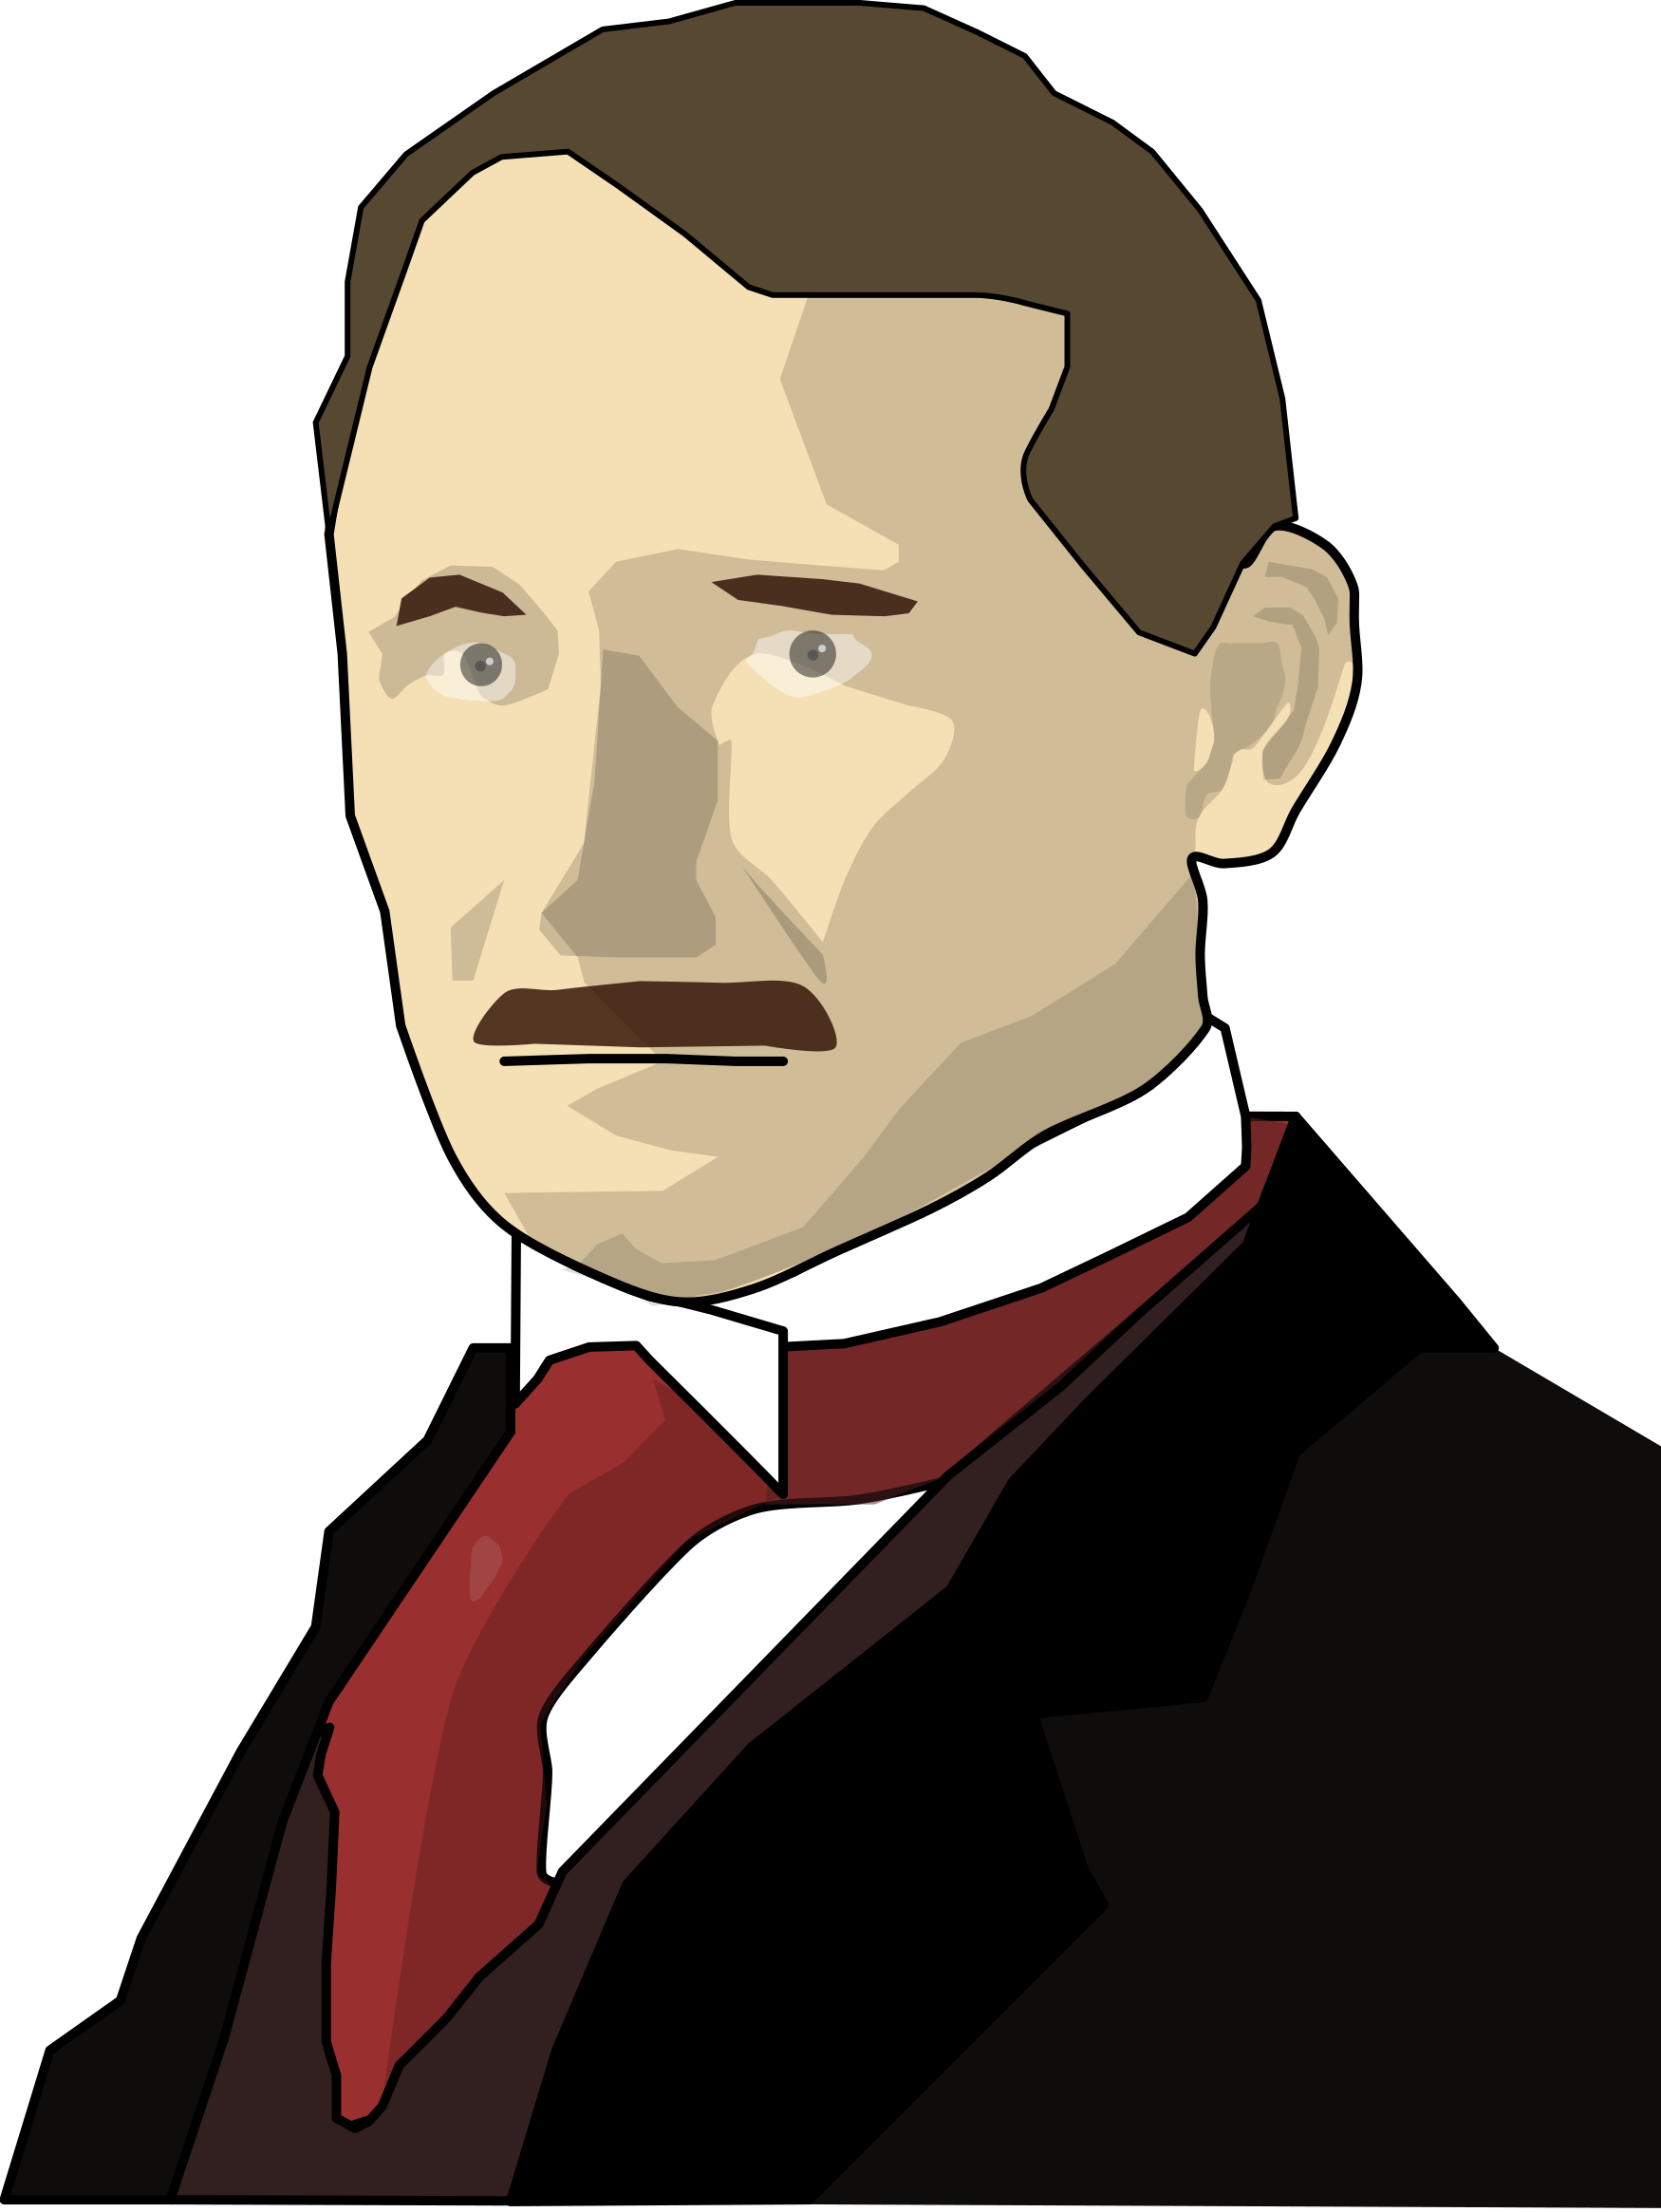
\includegraphics[width=0.3\textwidth]{winslow_friendly_flipped.png}
	\label{winslow:icon}
	\caption{Winslow Logo}
\end{wrapfigure}


The program that shall implement the requested features listed by \autoref{requested-features} is being called Winslow.
This name refers to Frederick Winslow Taylor who was an American mechanical engineer and one of the first management consultants in the 19th century\cite[wiki:winslow].
Both strive to make people's work more efficient.


\section{Common Terminology}
\label{winslow:terminology}

This chapter explains the meaning of words and terminology used later on.
It is crucial that every reader has the same understanding for the words used so that there are no wrong assumptions, expectations or surprises.

The root of a work item is called project.
A project will usually refer to one video footage that shall be processed.
Each project has its exclusive directory for input, output and intermediate files, called workspace.
Furthermore a project as an author and possibly participants, that can help in steering and monitoring the processing.
To do so, there is always a pipeline assigned to a project.

A pipeline consists of at least one but usually multiple stages that can at least be processed linearly - one after the other.
Furthermore, a pipeline can define environment variables that valid for all stages within the stage.

A stage is the smallest work unit that can be executed.
A docker image\autoref{docker:image} is specified as execution environment as well as further stage specific environment variables, command line arguments and hardware requirements (such as CPU cores, GPUs and minimum available RAM).
This enables a stage to use a common image as well as to specify very precisely how to process the data.

In addition, stages and pipelines can be distinguished in a active, running or completed stage or pipeline and a definition.
A stage definition specifies the above mentioned presets - allowing the user to adjust details just before submission - to create multiple stages from, while a running or complete stage has all information of what is or was executed and allows no further alteration.
For pipeline definitions this is similar, a pipeline definition can be used to specify a common order of execution.
Once assigned to a project, the project can freely adjust and change its instance of the pipeline.

\todo{execution node}
\chapter{\todo{Aims and Objectives}}
\label{requirements}

This chapter works out the desired capabilities of the software and then lists the resulting requirements.
Requirements help to keep track of whether the software covers all customer needs and wishes.
They also help during development to keep track of the progress and estimate the time required to implement the remaining requirements.

\todo{not complete, not anti-agile: it specifies the basic needs and expectations at the beginning}

\requirement{mgmt:create:pipeline}{1110}{Define a new Pipeline}{
	The user must be able to create a new pipeline definition.
	Only valid definitions must be accepted.
	A valid pipeline definition has a name and must contain at least one stage definition.
}
\requirement{mgmt:update:pipeline}{1120}{Update an existing Pipeline}{
	The user must be able to see and modify an existing pipeline definition.
}
\requirement{mgmt:delete:pipeline}{1130}{Delete an existing Pipeline}{
	The user must be able to remove an existing pipeline definition.
	Deleting a pipeline definition must not break and therefore must not prevent associated projects from further execution.
}
\requirement{mgmt:list:pipeline}{1140}{List all Pipelines}{
	The user must be able to retrieve a named list of all existing pipeline definitions.
}

\requirement{mgmt:create:project}{1210}{Create a new Project}{
	The user must be able to create a new project.
	Only valid projects must be accepted.
	A valid project has a name and must be using an existing pipeline definition.
}
\requirement{mgmt:update:project:pipeline}{1220}{Update the Pipeline of a Project}{
	The user must be able to change the pipeline definition an existing project is based on.
}
\requirement{mgmt:update:project:name}{1230}{Update the Name of a Project}{
	The user must be able to update the name of a project.
}
\requirement{mgmt:update:project:labels}{1240}{Updating Tags of a Project}{
	The user must be able to add and remove tags to and from an existing project.
}
\requirement{mgmt:delete:project}{1250}{Delete an existing Project}{
	The user must be able to delete a Project.
	Deleting a project must delete all associated files, directories and configuration files.
}
\requirement{mgmt:list:project}{1260}{List all Projects}{
	The user must be able to retrieved a named list of all existing projects.
}

\requirement{files:upload}{1310}{Upload Files}{
	The user must be able to upload files into the scope of a project, so that further stage execution is able to retrieve said file.
}
\requirement{files:download}{1320}{Download Files}{
	The user must be able to download files that are within the scope of a project.
	Said files can be files that were previously uploaded by the user or are results of executed stages.
}
\requirement{files:list}{1340}{List Files}{
	The user must be able to retrieve a list of files associated with a project.
}

\requirement{exec:start:stage}{1410}{Start a Stage}{
	The user must be able to start a new Stage for a project.
	Any Stage defined in the associated Pipeline Definition is considered a valid choice.
	The user shall be able to choose whether the following Stages shall be executed automatically or the pipeline shall be paused upon completion.
}
\requirement{exec:pause:stage}{1420}{Pause a Pipeline}{
	The user must be able to mark a running Pipeline of a Project to be paused before executing the next Stage.
}
\requirement{exec:resume:stage}{1430}{Resume a Pipeline}{
	The user must be able to resume paused Pipelines.
}
\requirement{exec:abort:stage}{1440}{Abort a running Stage}{
	The user must be able to commit an abort request for a running Stage.
	An aborted Stage shall be considered failed and further Stage execution shall be paused.
}
\requirement{exec:inspect:logs}{1450}{Inspect logs of a Stage}{
	The user must be able to see log messages produced by a selected Stage as well as to that stage associated system events.
}
\requirement{exec:inspect:state}{1460}{Inspect state a Stage}{
	The user must be able to retrieve the state ('RUNNING', 'PAUSED', 'SUCCEEDED', 'FAILED') for all stages of a project.
}

\requirement{node:monitor:cpu}{1510}{Monitor CPU usage}{
	The user must be able to retrieve the CPU utilization of all known nodes.
}
\requirement{node:monitor:ram}{1520}{Monitor RAM usage}{
	The user must be able to retrieve the RAM utilization of all known nodes.
}
\requirement{node:monitor:netio}{1520}{Monitor Network IO}{
	The user must be able to retrieve the Network IO utilization of all known nodes.
}



\section{Top Level Requirements}

\section{Requirements}

\subsection{Managing Pipelines and Projects}
\begin{itemize}
	\reqItemL{mgmt:create:pipeline}
	\reqItemL{mgmt:update:pipeline}
	\reqItemL{mgmt:delete:pipeline}
	\reqItemL{mgmt:create:project}
	\reqItemL{mgmt:update:project:pipeline}
	\reqItemL{mgmt:update:project:name}
	\reqItemL{mgmt:update:project:labels}
	\reqItemL{mgmt:delete:project}
\end{itemize}

\subsection{Managing Resources and Workspaces}
\todo{what about res/workspace/init directories}
\begin{itemize}
	\reqItemL{files:upload}
	\reqItemL{files:download}
	\reqItemL{files:list}
\end{itemize}


\subsection{Managing and Monitoring Executions}
\begin{itemize}
	\reqItemL{exec:start:stage}
	\reqItemL{exec:pause:stage}
	\reqItemL{exec:resume:stage}
	\reqItemL{exec:abort:stage}
	\reqItemL{exec:inspect:logs}
	\reqItemL{exec:inspect:state}
\end{itemize}

\subsection{Monitoring Nodes}
\begin{itemize}
	\reqItemL{node:monitor:cpu}
	\reqItemL{node:monitor:ram}
	\reqItemL{node:monitor:netio}
\end{itemize}

\subsection{Derived Requirements}
Requirements that are derived by looking at other requirements.


\todo{functional vs nonfunctional}

Die hier gelisteten funktionalen Anforderungen beschreiben das gewünschte Verhalten des
Systems \cite[155]{goll2012methoden}.

Nichtfunktionale Anforderungen zeigen im Gegensatz zu funktionalen Anforderungen Rah-
menbedingungen bei der Umsetzung des Systems auf \cite[155]{goll2012methoden}.



\chapter{System design}

In this chapter the previously collected information is used to design the system in detail.
The decision making process for that is documented here as well.

%\todo{mention? decentralization aspects?}

\section{Environment}

All Winslow instances are supposed to run inside a Docker container (as requested in \autoref{workflow:desired:docker}).
The hosts will be Ubuntu or Debian Linux Servers of which some will have one or multiple GPUs.
There will be no graphical user interface available on these servers.

The decision to implement Winslow in Java was made early on.
This has three main reasons, first, the developer is experience in Java development, the server side web framework used is a Java library (see \autoref{design:springboot}) and the company this implementation is for has a focus on Java development.
This means if the system is successful, maintenance and possible extensions might be authored by another developer who has probably knowledge in Java development as well.
% \todo{.cleanup}

%\todo{env: shall be executed on ubuntu/debian linux servers, Docker}

\section{Storage Technology}

Organizing and accessing data is one of the main concerns for Winslow.
In almost all use cases, multiple instances will need to access the storage.
It must therefore be accessible from remote and by multiple Winslow instances simultaneously.
For that, the following technologies are reviewed: NFS or SMB/CIFS (\autoref{analysis:storage:organisation}),  GlusterFS (\autoref{glusterfs}), SeaweedFS (\autoref{seaweedfs}), OpenIO (\autoref{openio}), dCache (\autoref{dcache}) and HadoopFS (\autoref{hadoopfs}).

The following criteria were used for comparison.
The scoring system provides points from 0 to 3, in which 0 means the best solution and 3 the worst.
The points of the individual categories are added together, the lowest overall score shall then point to the best solution:

\begin{itemize}
\item \textbf{Installation Overhead}:
How hard and extensive is the installation?
Is there a good documentation?
Is the package provided from within the main repository of Ubuntu, Debian, or alternatively, does it provide any other form of easy installation?
Scoring 0 for installation through the main repository, 1 for an external repository, 2 for a distribution specific archive, 3 for any other installation solution.

\item \textbf{Dependencies}:
Are further services required for operation? 
How hard are they to setup?
Do they need any additional configuration?
Scoring 0 for no further dependencies, 1 for dependency requirements but without the need of manual configuration,  2 for dependencies that require manual configuration, 3 for dependencies that need to be installed manually and require manual configuration.

\item \textbf{Single Point of Failure}:
Is the solution decentralized and is it failure resilient?
Is it site- or rack-aware or provide replication mechanisms to compensate?
Scoring 0 for completely decentralized, 1 for no direct SPoF but with a dependency on a centralized backend, 2 for a mostly centralized solution but with load balancing approaches, 3 for no single point of failure mitigations.

\item \textbf{Docker integration}:
How easy is it to integrate with Docker?
Scoring 0 for native support, 1 for native but non-trivial support, 2 for support through additional exports facility, 3 for non-trivial solution.

\item \textbf{Failure concerns}:
Are there any noteworthy concerns?
Was an early local test successful and reliable?
Is it a known technology or \enquote{proven in use}?
Who is developing it and what are the support guarantees?
Scoring 0 for commonly used and no concerns, 1 for minor concerns, 2 for major uncertainty, 3 for abandoned technology.
\end{itemize}

In \autoref{comparision:storage} the results are displayed:

\begin{table}[H]
	\begin{tabular}{|l|c|c|c|c|c|c|}\hline
				& NFS S.& SMB/CIFS S.& GlusterFS & SeaweedFs	& dCache 	& HDFS \\
		\hline
		Inst. 	& 0 	& 1 		& 0 		& 2 		& 3			& 1 \\
		Dep. 	& 1 	& 0			& 0 		& 0 		& 3 		& 1 \\
		SPoF 	& 2		& 3			& 0			& 2 		& 0			& 0 \\
		Docker 	& 0 	& 2 		& 2 		& 3 		& 2 		& 3 \\
		Fail.	& 0		& 0			& 1			& 2			& 2			& 0 \\
		\hline \hline
		Score 	& 3		& 6			& 3			& 9			& 10		& 5 \\ \hline
	\end{tabular}
	\caption{Failure concern comparison of storage technologies}
	\label{comparision:storage}
\end{table}

The worst scoring tool in this comparison is dCache.
The installation overhead, missing documentation and uncertainty on reliable operation is too high for this project (see \autoref{dcache}).

For similar reasons SeaweedFs is placed second worst.
Local tests could not access SeaweedFs reliable when a node failed and there is no trivial support for Docker nor does it provide an NFS export.
Using it would require each started container to be manipulated so that the first operation is mounting the storage with a custom binary and through a FUSE\footnote{Filesystem in Userspace} mount.
The tool also seems to be developed by a single person which introduces further uncertainty about reliability and support in the future.

HDFS and SMB/CIFS seem to be no terrible choice, but no especially good one either in this use case.

The two best scoring storage solutions are a simple NFS share and GlusterFS.
While GlusterFS provides replication and decentralized access, a NFS share scores with its simplicity.
The idea is to start with a plain NFS share for Winslow which can natively be utilized by Docker as volume mount and to revisit later whether the need for replication and decentralization persists.
Because of the NFS export feature of GlusterFS, Winslow could then easily switch to GlusterFS.



\section{Execution Management}

As noted in \autoref{analysis:layer_1}, the central business logic is to decide on when and to issue stage executions.
Generally speaking, there are two approaches when executing jobs: local or remote. Both will be discussed next.

In the remote approach, the job is executed on a machine that is not the same that has the responsibility to manage the process.
Continuous Integration (CI) platform Jenkins\cite{jenkins:main} does use this approach.
A so called slave node (Jenkins) is contacted through a native interface (SSH for Linux servers) to transfer resources and to start the job process.
In this scenario, the CI instance requires and stores login credentials for every remote machine to be able to login whenever needed.
The system administrator has to create a new user accounts on the remote machines, install required programs and prepare the environments.
One big risk for this approach is that in case of any security breach on the central CI instance, the attacker is also able to login on all remote machines.

GitLab\cite{gitlab:main} follows a more local approach, where the system administrator has to manually install the GitLab Runner on machines that are then able to connect to GitLab and execute jobs.
This runner is responsible in pulling jobs, executing them locally, monitoring and reporting back the outcome.

Winslow is going to follow the local approach.
On each physical machine that is supposed to provide compute resources, Winslow needs to be installed.
The installation is expected to be easy, as is based on starting a prepared Docker image.
An election between the Winslow instances is selecting the most fitting hardware for a stage execution (see affinity and aversion in \autoref{election:affinity_and_aversion}).
It is expected that each instance can judge this best on its own, as it knows which resources are available.
Work is distributed to an executor as it is detected.



\section{Event Synchronization and Communication}
\label{design:synchronization}

\begin{comment}
kafka does what? persist events and provides them in an order(?), cant Winslow do this itself, so that no further dependency is required?

\todo{.}
https://docs.microsoft.com/de-de/azure/architecture/microservices/design/interservice-communication


raw TCP (how to connect, centralized? star? tree?) centralized works towards -> centralized master node
broadcast?
microservice REST
event bus? kafka
messaging queue mqtt
NFS provides filesystem, filesystems are kind of standardized

https://kafka.apache.org/protocol
\todo{.}
\end{comment}


As discovered in \autoref{analysis:layer_2}, there is the need for event synchronization across all Winslow instances.
Without proper coordination, race conditions could cause stages to be started multiple times simultaneously, corrupt workspaces, configuration or project files.
While starting too many stage executions are only wasting resources, data corruptions can lead to unrecoverable damage.

There are multiple ways to exchange data between systems that do not share the same process or machine.
The most flexible implementation can be achieved by implementing a custom protocol on a raw TCP socket which allows to exchange blobs (Binary Large Objects) between exactly two nodes.
For a blob or message to reach all nodes, a connection to every other node, a centralized broker, another topology such as a tree structure or broadcast messages would be required.
Because this in itself seems to be a complex subject, third party alternatives were investigated.

Apache Kafka\cite{kafka} is one such alternative.
It is open source, distributed and is focused on providing a system wide ordered data and event stream that can be persisted over a certain time period.
But as every third party service, it introduces a dependency on the project.
Not only in regards to interfacing and driver implementation, but also for maintenance and setup.
Each Winslow Image would require to be shipped with a pre-configured Kafka service and the administrator must ensure that these services can reach each other - in addition to the storage solution.

Instead, it would be quite elegant, if an already planned connection between all Winslow instances could be reused for this, which could eliminate the need for third party dependencies here.
For now, only a common storage is required.
Re-using this as communication channel, a mechanism must be found to give each occurring event a sequence number, that is unique system wide.
New events would not be allowed to be propagated by an instance before it processed all previous events.
With this idea in mind, messages that can be used coordinated all required actions are defined next.

\begin{comment}

\todo{ACID in fundamentals?}
ACID, which stands for Atomicity, Consistency, Isolation and Durability, describes the needs a database must fulfill so that it does not suffer from side effects or data corruption when executing queries.
A series of changes might not be allowed to be intercepted (atomicity), must see and result in consistent data, is not allowed to interfere with simultaneously executed queries and guarantees that once completed successfully, is in fact persistent and will not be lost (durability).

\todo{filesystem is close}

\todo{DB principles: ACID}

\todo{...}

\todo{requires common a way to exchange messages}

\todo{all messages - called events - are published to all nodes}

\todo{using file system as bus}

\todo{clear and globally same order of events}

\todo{events consist of an id, command, time, duration, subject and issuer}

\todo{events might have a duration}

\todo{unspoken requirement: all nodes share the same clock - or one with very little drift}

\todo{usage as synchronization primitive}
\end{comment}

\subsection{Messages}
\label{message:grace_period}

To coordinate the Winslow instances, the messages will be exchanged through the common event bus, which broadcasts every message to all instances.

Because this is a multi instance system which can suffer partial failure, all multi-part operations have to have a timeout attached, so that a failure is detectable.
Without this timeout, one could not detect the absence of a finish signal for a multi-part operation, which could potentially block further operations for forever.

To account for transmission delay and slight clock offsets an additional time padding is granted.
Because of the non-requirement for real-time scheduling this can generously be set to 5 seconds.

All exchanged messages must share a common structure, which is listed next:

\begin{itemize}
	\item \textbf{issuer}: The id of the Winslow instance that published the message
	\item \textbf{command}: The state change request (described a bit further below)
	\item \textbf{subject}: What the command is about to change
	\item \textbf{timestamp}: The time of when the message was issued
	\item \textbf{duration}: Optionally, a non zero time period of the expected duration
\end{itemize}

With this message structure definition, the following commands can be used:

\begin{itemize}
	\item \textbf{LOCK}: Locking a resource, commonly a project.
	A lock is exclusive to the issuer and can only one at a time can be granted for a subject.
	\item \label{message:extend} \textbf{EXTEND}: Updating an ongoing operation by extending the timeout.
	This can be used to signal that a lock is still required although its timeout is about to be reached.
	The duration of the original event is extended and therefore the timeout is pushed back.
	The issuer must be the same as the issuer of the operation that is referred to.
	\item \textbf{RELEASE}: Releasing a locked resource.
	The issuer must be the same node as the one that issued the \textbf{LOCK} previously.
	\item \textbf{KILL}: Non-gracefully stop an operation or destruction of a lock.
	This signals that an operation shall be stopped or that the lock shall be released immediately.
	This can be used to abort an running stage execution.
	\item \textbf{ELECTION\_START}: Signals that an election for a stage execution has started.
	The signal must refer to an project that can make progress.
	\item \textbf{ELECTION\_PARTICIPATE}: Signals that the issuer node is capable of executing the next stage of the mentioned project.
	It also includes a scoring for the affinity and aversion (more details in \autoref{election:affinity_and_aversion}).
	This message must always refer to a valid election.
	\item \textbf{ELECTION\_STOP}: Signals that an election has finished.
	The participator with the best score is now allowed execute the next stage of the referred project.
	This is signal is only allowed to be issued by the same node that started the election process.
\end{itemize}

\subsection{Synchronization}

In a file system two files with the same name are not allowed to exist in the same directory, which is ensured by the filesystem.
This can be used when publishing events in a common directory: a by all instances followed sequence number is used as file name.
Publishing a new event will fail, if there already exists a file for that sequence number.
Watching the directory will then also result in a stream of ordered events.

To publish an event, a naive implementation would first check the directory for the next number in the sequence and to create it, if it was not found.
But this has a potential race condition: between checking for the file and creating it, another instance could have created the file.
Luckily, the POSIX standard provides a flag when creating files, that will expose this conflict by returning an error, if \enquote{Both O\_CREAT and O\_EXCL are set, and the named file already exists}\cite{gnu:open}.
This mechanism is also exposed in Java by calling \javacinline{Files.write(..)}\cite{javadoc:files:write} with \javacinline{StandardOpenOptions.CREATE\_NEW}\cite{javadoc:standard_open_options:create_new}.
The behaviour of publishing an event can therefore be summarized with \autoref{event:synchronized_publish}:

\begin{figure}[H]
	\centering
	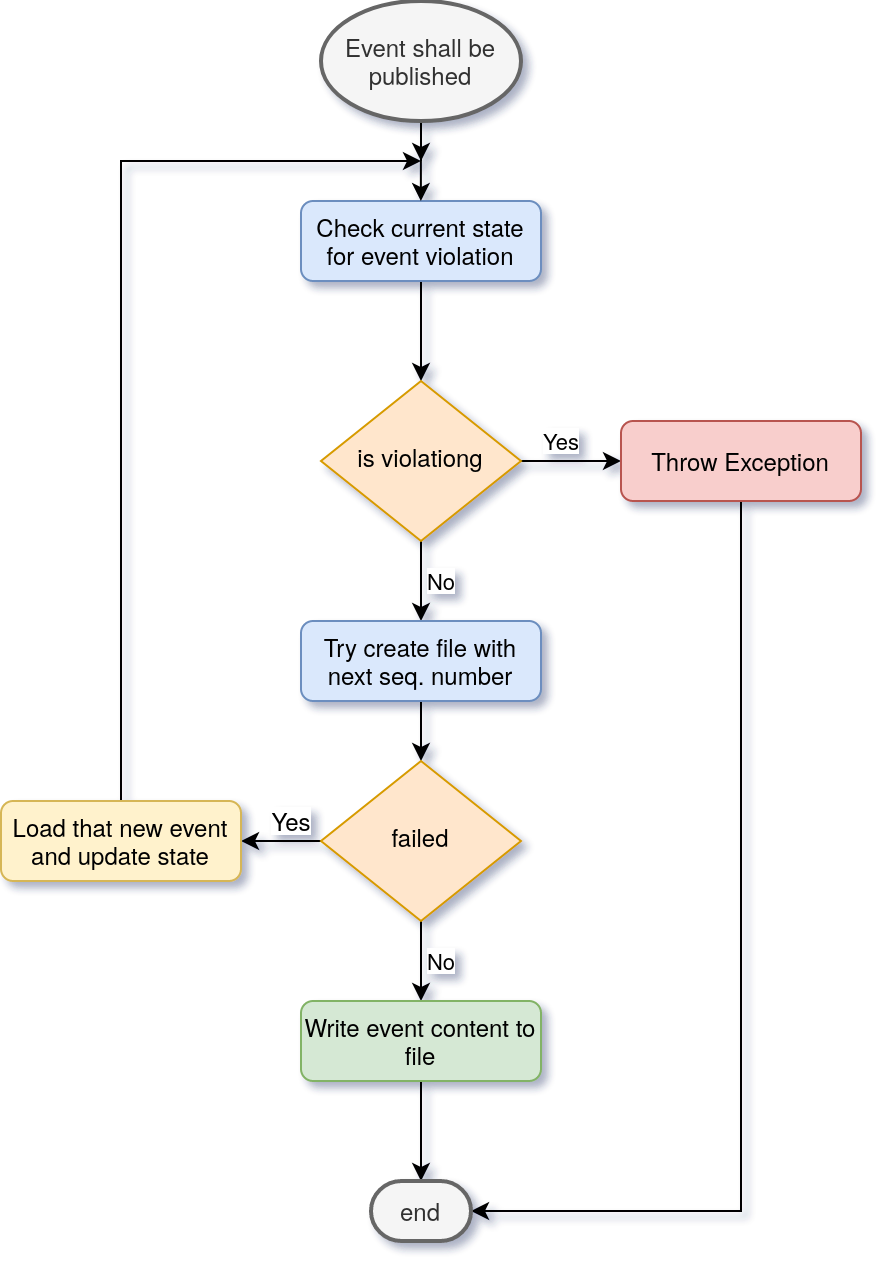
\includegraphics[width=0.65\textwidth]{event_publishing.png}
	\caption{Event publishing process}
	\label{event:synchronized_publish}
\end{figure}

Every Winslow instance is responsible for keeping track of all global states and check before publishing a new event whether the state would be violated by this event.
If it is not, it will try to publish it by creating a new file with the next sequence number.
If the file already exists, another instance did publish an event in the meantime.
This externally published event must then be loaded and the global state updated before a new attempt in publishing the original event can be made.
Eventually, this will either lead to successfully publishing the event or failing due to state violation - for example trying to lock a project that is already locked.


This synchronization mechanism ensures that each event is only published if it is not violating any constraints, such as locking resources that are already locked.
It also allows for multiple locks and elections to happen concurrently, as long as there is no overlap.

\begin{figure}[H]
	\centering
	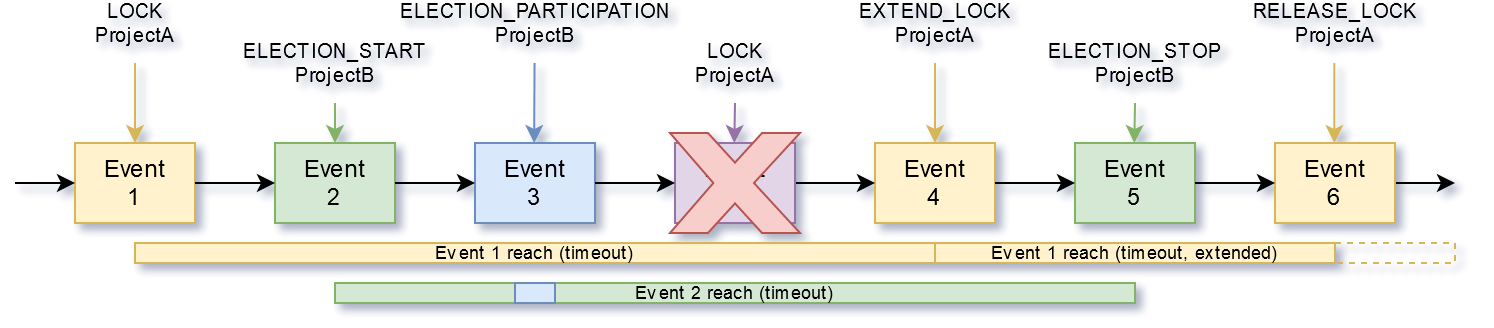
\includegraphics[width=1.0\textwidth]{events.png}
	\label{winslow:com:events}
	\caption{Sample event and lock series with lifetimes}
\end{figure}

In \autoref{winslow:com:events} a series of events, their sequence number and commands are shown.
The coloured rectangles below shows the duration of their lifetimes.
The crossed-out event is violating the constraint that a resource can only be locked by one instance at a time: the yellow lifetime in this case.
Because of this violation the even is never published to the event bus, which is demonstrate with the sequence number of the next event not skipping the number 4.

\section{Docker interface}


To interface with the Docker daemon a driver implementation is needed.
It needs to on container creation commands with a set of environment variables and the path to a prepared workspace.

Docker provides a REST API\cite{docker:api} for third party libraries as well as implementations in Go and Python.
There is no official Java API implementation.
This means, either a third party Java library must be used, the REST calls that are required have to be implemented within this project or another alternative must be found.
The Docker REST API is very expressive which is a reason to not implement the REST calls within this project.

As it turns out, the Nomad Project, which was already investigated in \autoref{nomad}, provides a library with a thin abstraction layer and lots of reasonable default values.
It also includes support to create container that use the Docker plugin from Nvidia\cite{nvidia:docker_plugin}.
This allows attaching GPUs to a container without the need of listing all libraries and device files manually\footnote{If you are interested in how tedious this could otherwise become, see \url{https://github.com/hashicorp/nomad/issues/3499\#issuecomment-364214506}}.
The scheduling capabilities of Nomad are not used because the focus of nomad does only overlap partially with the needs of Winslow.
A job is expected by Nomad to rerun, moved to different hosts and - in the service mode - scaled as it seems needed.
The control of where the job is executed is then lost, which is not acceptable when different firewall rules apply to all Winslow instances and a judgement for the best hardware utilization was already made.
Furthermore, when using GlusterFS or another cloud storage or compute capabilities, the network share is not always reachable through the same proxy for every node.
The lack of control could then cause stage execution failures due to unreachable workspaces.
Nomad will therefore only be used in the local Winslow container as thin layer to interface with an enriched Docker API.

%\todo{because: nomad focuses on scheduling multiple instances of a load balanced service, lack of control on where it is spawned, additional communication channels required -> firewall/admin/maintanance, interfer with further extenstions cloud like cloudstore and GlusteFS because a 'randomly' by nomad chosen node would require access to the storage which might not be visible to all executions nodes through the same path}.


\section{Directory Structure and Organization}

This section describes the organization of the working directory for the Winslow instances.
Because a common network share is required by Winslow for event synchronization and the projects' workspaces, this was further extended to share the configuration and project files as well.
This has the very nice side-effect, that there is no real setup to do when installing a new Winslow instance\footnote{\autoref{appendix:winslow_installation} lists the complete installation script for a new Winslow instance}, it just needs access the to working directory.

For the configuration files, a principle found on Unix and Linux systems was applied: human readable text files.
For complex structures YAML formatting is used, while for simple key value files property formatting is used.
This makes understanding the system state easier when debugging in error scenarios.

\subsection{Winslow working directory}
\label{design:winslow:workdir}

A brief summary of the by all instances shared working directory:

\begin{itemize}
	\item \monospaceinline{logs}: The location for stage log files.
	This includes system events and the console output with timestamps.
	The file name is formatted as \\
	\monospaceinline{<project-id>-<stage-number>-<stage-name>}.
	\item \monospaceinline{pipelines}: Pipeline definition file (YAML) are located here.
	\item \monospaceinline{projects}: Project definition files (YAML) are located here.
	\item \monospaceinline{resources}: The globally available input resources, see \autoref{stage:workspace}.
	\item \monospaceinline{run/events}: The directory used to synchronized events, see \autoref{design:synchronization}.
	\item \monospaceinline{run/nodes}: The directory used to publish node utilization, see \autoref{design:monitor_resources}.
	\item \monospaceinline{settings}: The directory used to share common configurations, currently this only contains a global environment variable configuration.
	\item \monospaceinline{workspaces}: The per project specific workspaces are located here, see \autoref{stage:workspace}.
\end{itemize}

Because the files in \monospaceinline{run/events} and especially \monospaceinline{run/nodes} are very temporary, the NFS server locates these in shared memory (\monospaceinline{/dev/shm}) to reduce stress on IO and unnecessary wear on SSDs.
%Thanks to the synchronization and locking mechanism (presented in \autoref{design:synchronization}), the working directory can shared between all Winslow instances.

\subsection{Stage storage}
\label{stage:workspace}

The storage organization for a project and its stages had a few unexpected concerns raised.
%Thinking about the storage organisation for the pipeline and its stages, a few expectations and concerns arise.
First of all, to redo a stage, one needs to be able to access the files that were the result of one, two or multiple stages before.
Sometimes a stage wants to access intermediate data produces by multiple previous stages.
Next, the input video footage needs to be accessed by multiple stages throughout the pipeline execution.
Finally, some stage results are not intermediate but do already present some final results.

The first and second concern can be solved by providing a workspace directory for each stage, that is copied from the logically previous stage\footnote{the stage the new one is based on, this does not always need to be the numerical previous stage}.
Once the computation of a stage is completed, the workspace is considered immutable and only used to source new workspaces from.
This works fine for small intermediate results, but it does not work very well for large files - like the video footage.
This delays the start of the stage execution, requires unnecessary storage due to multiple copies and provides no benefits in an archival and version control sense, because the video footage is not altered.
So there needs to be another storage pool for input data, that is globally accessible and never changed: the global input storage pool.
Providing one further storage pool for final results (global output pool), concern number three and four are also solved.

Because the very first stage has no workspace to source its files from, on creation of the project a workspace directory for the \enquote{zeroths} stage is created.
The user can then provide the very first stage with a predefined and non-empty workspace if necessary.

This also solves te problem with delays due copy operations in NFS, which are performed client side.
This means, the client reads the input file and writes to the output file\footnote{Server-side copy has just been standardized for NFS 4.2\cite{nfs:ssc}}.
This operation does not only take unnecessary long but also utilizes all available network bandwidth which then cannot be used by other applications.

To ensure that the global input and the previous intermediate results are not altered, the Docker daemon is instructed to mounted them as read-only filesystems.
This also prevents bugs or errors from accidentality deleting unrelated files\footnote{\enquote{This so theoretical and will actually never happen in real life} proven otherwise: \url{https://github.com/valvesoftware/steam-for-linux/issues/3671}}.
\autoref{storage_organization} summaries all this:


\begin{figure}[H]
	\centering
	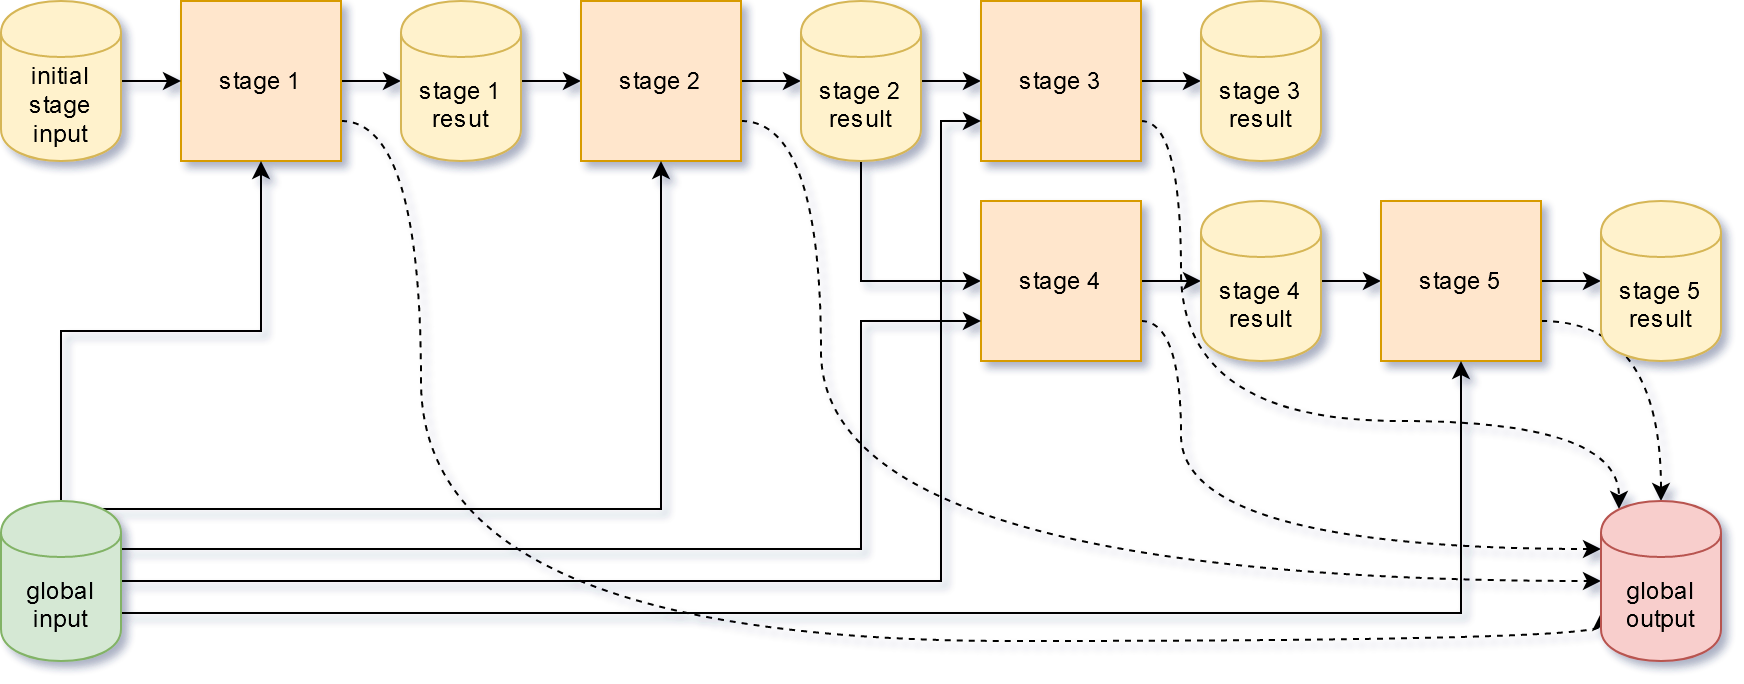
\includegraphics[width=0.9\textwidth]{stage-storage.png}
	\caption{Stages with their intermediate and global resource pools}
	\label{storage_organization}
\end{figure}

For a running stage the mounted directories looks like the following:

\begin{itemize}
	\item \monospaceinline{/input} is mounted read-only from \\ \monospaceinline{nfs-server:/winslow/workspaces/<project-id>/input}
	\item \monospaceinline{/output} is mounted with write permissions from \\ \monospaceinline{nfs-server:/winslow/workspaces/<project-id>/output}
	\item \monospaceinline{/workspace} is mounted with write permissions from \\ \monospaceinline{nfs-server:/winslow/workspaces/<project-id>/<stage-id>} \\
	and was created by the copying the workspace directory of the logically previous stage into it
\end{itemize}


%\todo{define logically previous stage -> previous stage on linear execution and ... when jumping around}
%stage execution does not need to depend on the result of the exact previous



\section{Job Scheduling and Election System}
\label{design:election}

Winslow has no ahead of time plan to schedule stage executions, the main reason for this that it is unknown how long a stage is about to take.
One could consider to build statistics to eventually be able to guess the duration of repeatedly executed stages, but this seems error prone, does not cover seldom executed stages and is in addition unreasonable complex.
%\todo{mention these complex scheduling techniques?}
Instead, the system is reacting to user submissions and on stages that have just completed.
For each new execution, an election is then held in which the winner will execute the stage.
Winslow instances that do not fulfil the resource requirements do not participate in the election.

\subsection{Affinity and Aversion}
\label{election:affinity_and_aversion}

To determine a winner, participants must be comparable.
Winslow uses a two factor scoring mechanism for that, in which it judges how efficient a node is going to be utilized (affinity scoring) and how many unused resources will be wasted (aversion scoring).
The instance with the highest affinity value out of the instances of the lowest aversion values wins.

This system was developed within this thesis but loosely inspired by Nomad\cite{nomad:main}, which also uses an affinity score\cite{nomad:affinity} but no aversion equivalent.
Instead of specifying this value in each job definition like in Nomad, Winslow derives it's values from the available resources and resource requirements.
This requires less user interference, prevents blocking unused hardware and still delivers good results, as will be discussed next.

For determining the affinity scoring only requested resource categories $c_i$ need to be considered.
Through the resource monitoring (see \autoref{design:monitor_resources}) the total resources $r_{c_{max}}$ as well as the reserved resources $r_{c_{in\_use}}$ are known.
For every requested resource by the stage definition $c1 .. cx$, the ratio between requested $r_{c_i}$ and available resources is calculated.
The lowest ratio, and therefore the most pessimistic value, of any category is used as the affinity score:

\begin{equation}
	\label{election:eq:affinity}
	\text{affinity} = \min_{c_1 .. c_x} \left( \frac{r_{c_i}}{r_{c_{max}} - r_{c_{in\_use}}} \cdot n_{c_x} \right)
\end{equation}

As seen above, every node can additionally apply a resource category specific multiplier $n_{c_x}$ for punishment or gratification.
This allows to fine tune the score on a per node basis.

For determining the aversion scoring, all by a node available resource categories $c1 .. c_a$ need to be considered.
In contrast to the affinity score, the highest ratio of any unused resource is used as aversion score, which is again the most pessimistic value.

\begin{equation}
	\label{election:eq:aversion}
	\text{aversion} = \max_{c_1 .. c_a} \left( \frac{r_{c_{max}} - r_{c_{in\_use}} - r_{c_a}}{r_{c_{max}}  - r_{c_{in\_use}}} \cdot n_{c_a} \right)
\end{equation}

The more resources are wasted - especially categories that are untouched at all - the worse the aversion score.

An example shall illustrate the scoring system.
Lets consider the following three execution nodes exist:

\begin{table}[H]
	\centering
	\begin{tabular}{|l|r|r|r|}\hline
		 & Free CPUs & Free memory & Free GPUs \\
		 \hline
		 Node 1 & 4  	& 16 GiB & 0 \\
		 Node 2 & 12 	& 58 GiB & 0 \\
		 Node 3 & 4 	& 50 GiB & 1 \\ \hline
	\end{tabular}
	\caption{Nodes to consider}
\end{table}

The following three stages executions shall be assessed:

\begin{table}[H]
	\centering
	\begin{tabular}{|l|r|r|r|}\hline
		& Req. CPUs & Req. memory & Req. GPUs \\
		\hline
		Ex1 & 2 & 16 GiB & 0 \\
		Ex2 & 4 & 48 GiB & 0 \\
		Ex3 & 4 & 16 GiB & 1 \\ \hline
	\end{tabular}
	\caption{Stage executions to consider}
\end{table}

The following table shows the resulting affinity and aversion score.
The winning node for is marked by the bold formatting.


\begin{table}[H]
	\centering
	\begin{tabular}{|l|r|r|r|}\hline
		& Node 1 & Node 2 & Node 3 \\
		\hline
		Ex1 & \textbf{0.5/0.5}	& 		  0.28/0.72	& 		  0.32/1.0 \\
		Ex2 & - 				& \textbf{0.34/0.67}& 		  0.96/1.0 \\
		Ex3 & - 				& - 				& \textbf{0.32/0.68} \\\hline
	\end{tabular}
	\caption{Affinity/Aversion score for every stage definition and node constellation that provides all required resources}
\end{table}

As shown in the example, the aversion score is important to prevent stages taking execution nodes that provide specialised hardware (such as GPUs) which is not required by the stage execution.
In this example, it prevent Ex2 to be scheduled on Node 3, which provides a GPU.

In comparison to just forbidding executions on nodes with hardware that is not used, in scenarios where all general purpose nodes have failed, are unreachable or stage execution has very little requirements, this system would still schedule executions.
But it tries as best as possible to prevent blocking unused resources, like Ex1 and Ex2 running on GPU nodes.

\section{Execution}

The execution of a stage is started on the Winslow instance that won the corresponding election.
It first locks the project, to re-read the configuration and to prevent any changes to in the meantime.
The workspace is being prepared (see \autoref{stage:workspace}), environment variables collected and the backend driver instructed to start the new container.
Any data logged to the containers' stdout or stderr is collected and written to a log file exclusive to this stage execution (see \autoref{design:winslow:workdir}).
System related events, such as errors pulling an image, exhausted resources or sudden aborts are also logged to this file.

A lock on the project is not held during all the time the stage is being executed, because it would prevent stages being enqueue and or prepared by a user in the meantime.
Instead, after successfully starting the new container and the log file has been created, a new lock pointing to the log file is created.
The currently executed stage is noted in the project file and then the lock on it is released.
As long as the lock for a log file is alive, no election for the project is allowed.

Once the container has stopped - and the stage has therefore either failed or succeeded - the lock on the project is acquired again to update the stage state.
After this, both locks are released, potentially triggering the next election.

\begin{comment}
\todo{affinity}
\todo{aversion}

Utilizing Event Bus for timely limited elections and to ensure that there are no concurrent election for a single project.

\todo{what about concurrent elections on multiple projects}

\todo{regarding locking: check for updatable, try to lock, check for updatable again, update, unlock}

\todo{on unlock: check updatable}



\todo{scheduling / job assignment/pull strategy}

\todo{graph displaying over time lock and election}
\end{comment}


\section{CPU, RAM and IO Monitoring}
\label{design:monitor_resources}

Monitoring the hardware utilization can be accomplished by parsing the contents of \monospaceinline{/proc/cpuinfo}\footnote{\url{https://www.kernel.org/doc/Documentation/cputopology.txt}}, \monospaceinline{/proc/stat}, \monospaceinline{/proc/meminfo}\footnote{\url{https://www.kernel.org/doc/Documentation/vm/hugetlbpage.txt}}, \monospaceinline{/proc/net/dev} and \linebreak\monospaceinline{/proc/diskstats}\footnote{\url{https://www.kernel.org/doc/Documentation/ABI/testing/procfs-diskstats} and \url{https://www.kernel.org/doc/Documentation/iostats.txt}}.
These special files in the \monospaceinline{/proc} directory are text files generated by the Linux kernel to summarize the current utilization\cite{linux:doc:proc}.

Each Winslow instance is repetitively reading and parsing these files and writing a summarized version to the shared workspace directory \monospaceinline{/run/node/<node-name>}.
An summary example can be seen in \autoref{appendix:run_nodes}.

\section{User Interface}
\label{design:springboot}

To display data on the user interface\footnote{Screenshots in \autoref{appendix:screenshots}}, REST requests are sent to the web-backend of Winslow.
To handle these requests and to serialize the responses Spring Boot\cite{springboot} is used by Winslow.

To not stress the event bus with lock requests caused by the user, all data retrieval operation open and read configuration files without locking them.
This bears the risk of reading incompletely written files, but as the user interface is not crucial to the system and as it must account for failed requests due to network issues anyway, this is considered acceptable.
The user interface would simple resubmit its request.
% \todo{ACID hazards ref?}

When modifying settings or triggering stage executions, the request handling must obey the locking rule to not introduce inconsistent state to the system (due to a dirty read\cite[2]{berenson1995a} that could occur without locking).
This means, on a HTTP POST request, the affected resource is being locked, updated and released.
The release will then trigger a Winslow instance to check the file for potentially starting an election.


%\todo{REST request, read only: no lock; for changes: POST -> LOCK -> update -> RELEASE, on RELEASE Winslow gets notified and checks whether the new configuration leads to a new stage execution}




\begin{comment}
\section{File system}

\todo{docker can auto mount nfs to container}

\subsection{Every node has a connection to every other node}

\subsection{Centralized broker}

\subsection{Tree hierarchy}

\subsection{outcome}




\section{Communication and Node Management}

The system that shall be developed, is supposed to spread jobs onto execution nodes as available.
There are two main approaches in nod management and job assignment.



\subsection{Centralized Management, Remote Execution}

In the central management approach, there is always exactly one leader at any given moment in time.
It is the responsibility of this leader to decide what to execute and where to execute it.

\subsection{Decentralized Management, Local Execution}

\subsection{Combinations worth noting}

stupid:
 - centralized management, local execution
 - decentralized management, remote execution
 
combination, decentralized + some remote slaves

\subsection{Architecture}

event based

common file system for communication because minimum requirements

stick to unix principles(list): simple, human readable intermediate format

voting/election by capabilities and 'will' of a node to run a stage

\todo{providing live hw utilization}

\todo{the whole properties thingy}

\subsection{Failure handling}
\todo{handling failed stages}

\todo{handling failed nodes}

\section{Communication/Event architecture?}

\section{Targeting capabilities}

\subsection{General thoughts}

\section{Planned}

\section{Implementation details}

\section{Synchronization, Locking, publishing events}

\section{REST for UI}



\subsection{Atomicy of (Unix) Filesystems}

\subsection{Atomicy and behavior of NFS in particular}

\subsection{Using as lock backend}

\subsection{Using as election backend}
\end{comment}




%\section{Agile development}

%\todo{.depends, maybe to shallow and not worth noting, dont forget to then ref to \autoref{fundamental:agile}}


\section{Continuous Deployment}

Winslow uses GitLab CI to continuously deliver runnable Docker Images after each git push.
Every code change triggers a new build pipeline, that builds and tests Winslow, packages all dependencies\footnote{Nomad and the Angular Web-Application} into a Docker image and pushes it to our in house private Docker Registry.
Broken code or failing unit tests will result in a notification for the developer and prevents the image from being published.

To update an execution node, the Docker container can simple be stopped and discarded.
The installation script\footnote{Which is displayed in \autoref{appendix:winslow_installation}} then pulls and starts the most recent image.
\chapter{Implementation notes}



\section{Execution environment}

\section{Continuous Deployment}

%\chapter{Things to solve / decide upon}

\section{Programming language}

\subsection{Java}
\subsection{Rust}
\subsection{Scala?}
\subsection{Go?}

\section{Docker image packaging?}
%\chapter{Implementation}

log strategy?

how to handle changes in configuration on a restart
 - how to sync with nomad
 - how to handle still running jobs on an now invalid configuration?
    - keep copy of old configuration?

\section{Orientation}

bash -> variable substitution

\section{No unexpected behavior}

no null, instead use Optional

lists are never null nor Optional but empty or filled instead

see de.itd.tracking.winslow.config.*

called defensive programming?
  - good to be error-resilient
  - bad in performance critical scenarios
  

%

describe the tool, what it is for, what it does, current workflow

The current workflow consists of the following steps:

- define reference points in one single frame through a user input

- track stationary reference points on all other frames

- estimate the camera position for each frame

- detect vehicles in all frames

- track detections and assign them to trajectories

- perform lane detection

- record a result video

- export trajectories to a csv-file

- create charts



As listed above, at least one stage must be able to process user-input. The

current progress must be observed and errors must be reported in an way, that

allows one to understand the circumstances for the cause of the error.

For easy and fast scalability, docker images shall be used to distribute the

binaries onto the nodes.


\section{Defining the Problem Space}

what is required / what shall the implementation be capable of from the view of the "user"

user interaction



\section{Analyzing the Problem Space}

describe scenarios the implementations must be able to handle in order to archive the requirements?

resource tracking
- global (read-only) input resources ("big" data files)
- per stage evolving project files
- might have some kind of version control?
- dynamically detect within a stage whether user input is required
- be able to continue / redo latest stage
- error / warning detection / tracking!
( [!a-zA-z]err[!a-zA-z])|( [!a-zA-z]error[!a-zA-z])
- web technology

- retrieve required binaries
- retrieve required resource files
- archive output files and logs

- persistence stage/state tracking of projects/pipelines/states

Problems to solve



- stages might have individual hardware requirements

- multiple stages might require the same hardware at the same time

- stages can depend on the result of another stage

- for scalability, it shall be easy to add and remove hardware-nodes

- the video files are large (4k footage), sending decoded frames (~25MB)

through the network might be unreasonable

- the definition of a pipeline shall be easy to understand for good

maintainability

- the hardware shall be used efficiently to achieve a high throughput

- docker images need to contain and provide all required libraries

- prevent stages from leaving other stages far behind?

- storage and distribution of intermediate results

- log collection




adding a new host
- instantiate docker image and mount config and docker socket?
- encrypt communication between control and worker?
- possibility for decentralization
- makes archiving logs and results hard


scenarios

define pipeline
- define gpu stage
- define cpu stage
- define required input assets
- define assets for each stage to be accessible in the next stage
- stages depend on other stages
- do it the other way around? set next stage?
- next stage + "parameters" (assets to keep/transfer)
- allows branching

upload resource file (video)
- ... upload <path> <name-at-remote>
- maybe to one common pool of resources?
- free disk space?

start pipeline
- select resources required by the pipeline
- start

go through stages until finished
- take care of cpu/gpu env requirements
- if no common pool of resources: concurrently copy assets to target machines
- archive 

maybe: halt at stage because of error / required user interaction
- allow continuation
- allow download / upload of assets into this stage
- free disk space?


easy installation and binary distribution
- docker image per pipeline stage?
- map management binary into docker -> exec
- requires standalone binary
- implicitly requires compatible libc env/unix system
- requires administrative (docker ) privileges


outputs of a stage are immutable after it has finished, stages using that data are working on a copy

nice to have: display progress captured from log (regex filter with multiple subjects/progresses per stage)

show time a stage is running

show estimated remaining time (based on captured progress)

todo list per project

project can run through multiple pipelines multiple times

nomad -> .deb archive?

deployment
- web
- controller
- third party / nomad

start
start from a certain stage
pause after a stage
redo a stage
change variables at a stage

%\include{chapters/ex4}
%\include{chapters/deliverables}

%---------------------------------------------------------------------
%--- Bibliography and appendices
%---------------------------------------------------------------------

\printbibliography
\addcontentsline{toc}{chapter}{Bibliography}

%\appendix
%% to utf8: ö
\chapter{Extra data}

		
\end{document}
